\section{Experimental Results}

\begin{figure*}[t!]
    \centering
    \begin{subfigure}[t]{0.5\textwidth}
        \centering
        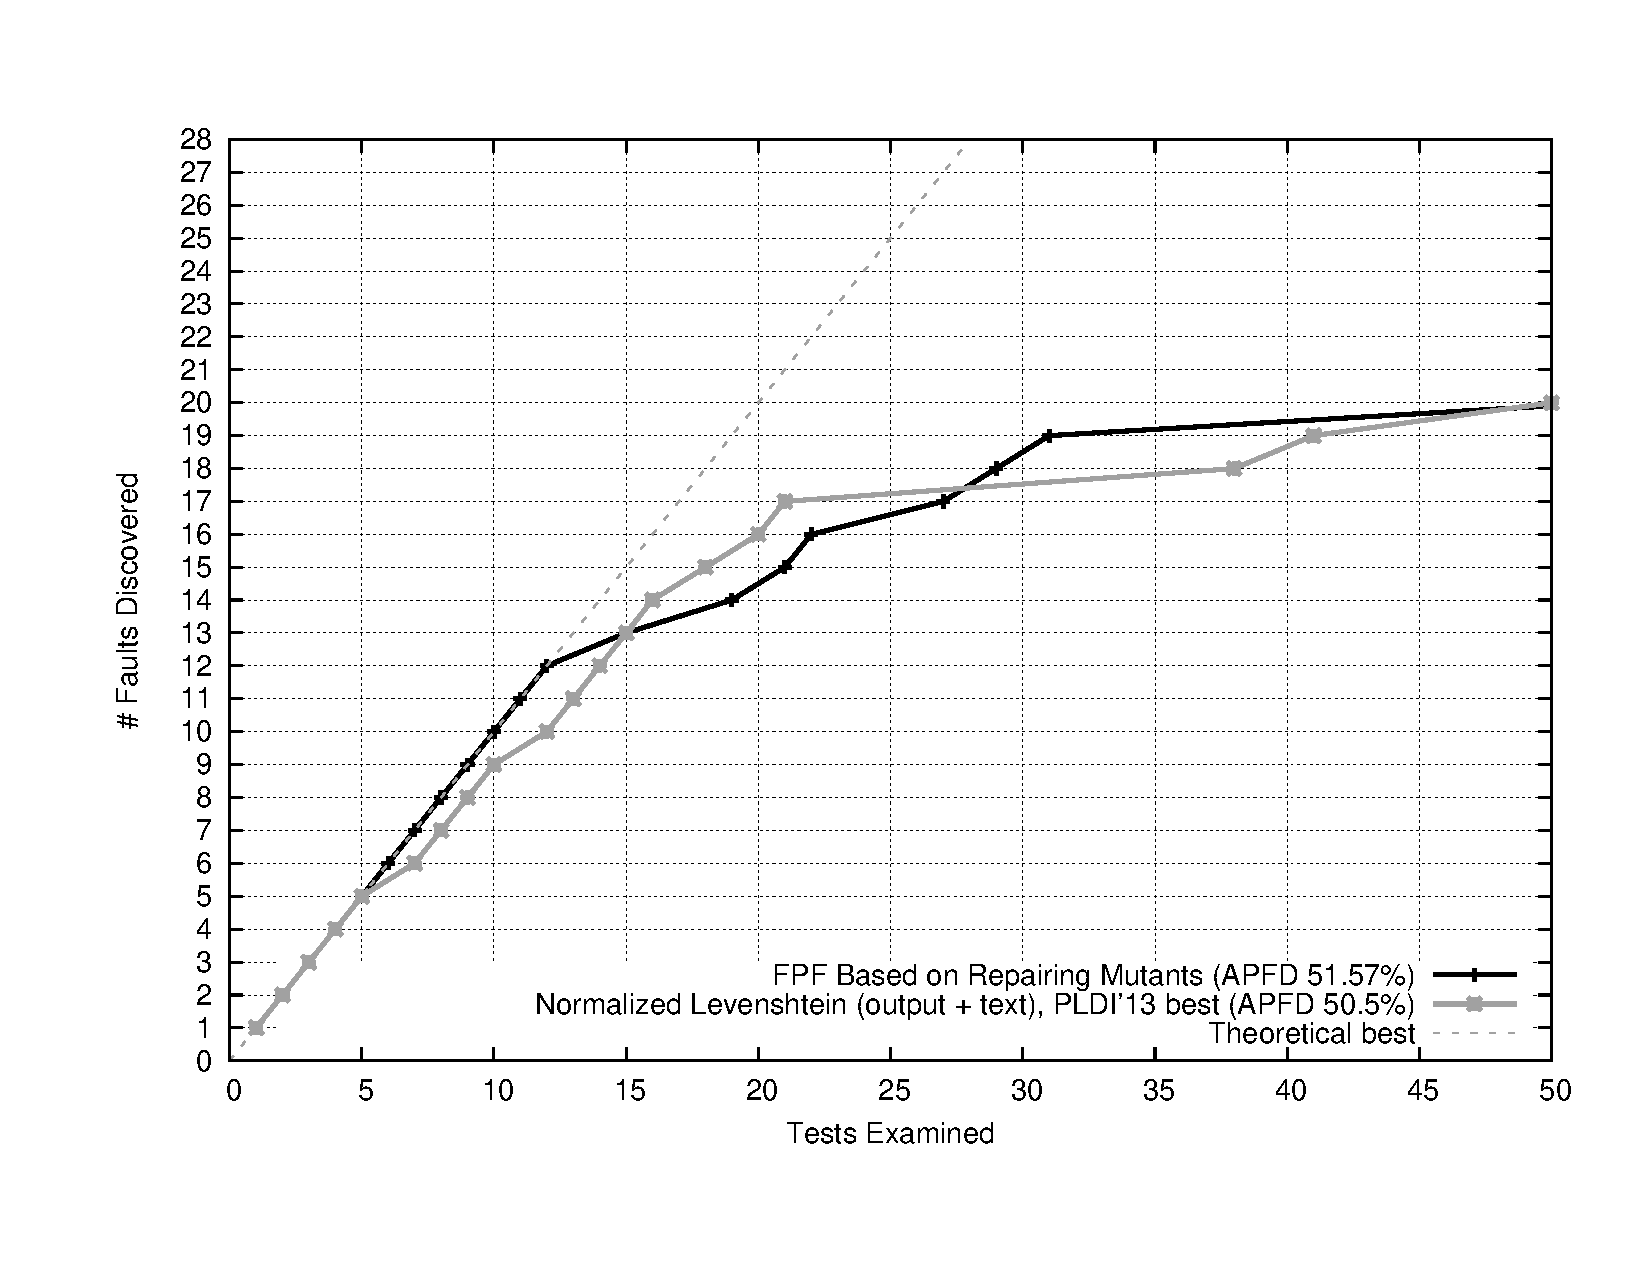
\includegraphics[width=1.02\textwidth]{jscurve}
        \caption{Discovery curves for SpiderMonkey 1.6 faults}
        \label{jscurves}
    \end{subfigure}%
    ~ 
    \begin{subfigure}[t]{0.5\textwidth}
        \centering
        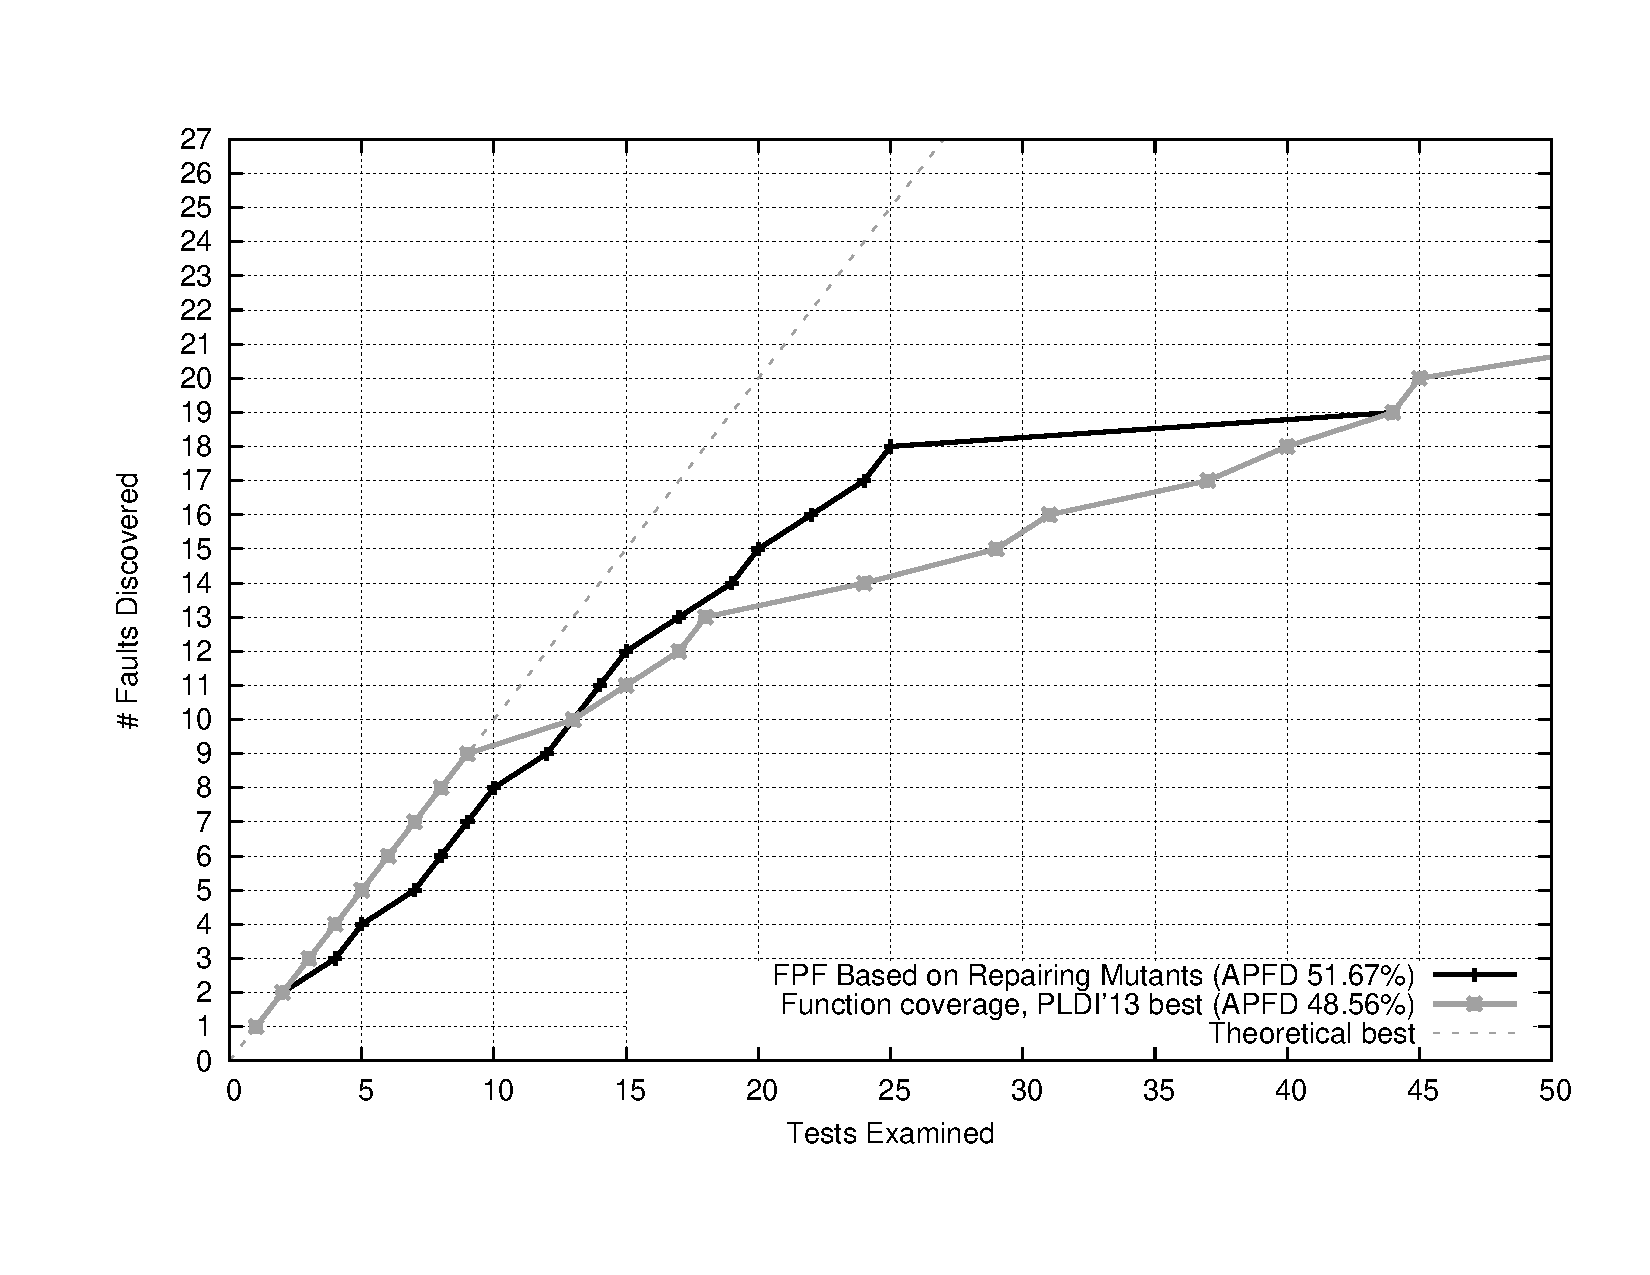
\includegraphics[width=1.02\textwidth]{gcccurve}
        \caption{Discovery curves for GCC 4.3.0 wrong-code faults}
        \label{gcccurves}
    \end{subfigure}
    \caption{Discovery curves compared to best curves from PLDI 2013}
\end{figure*}


%\begin{figure*}
%\centering
%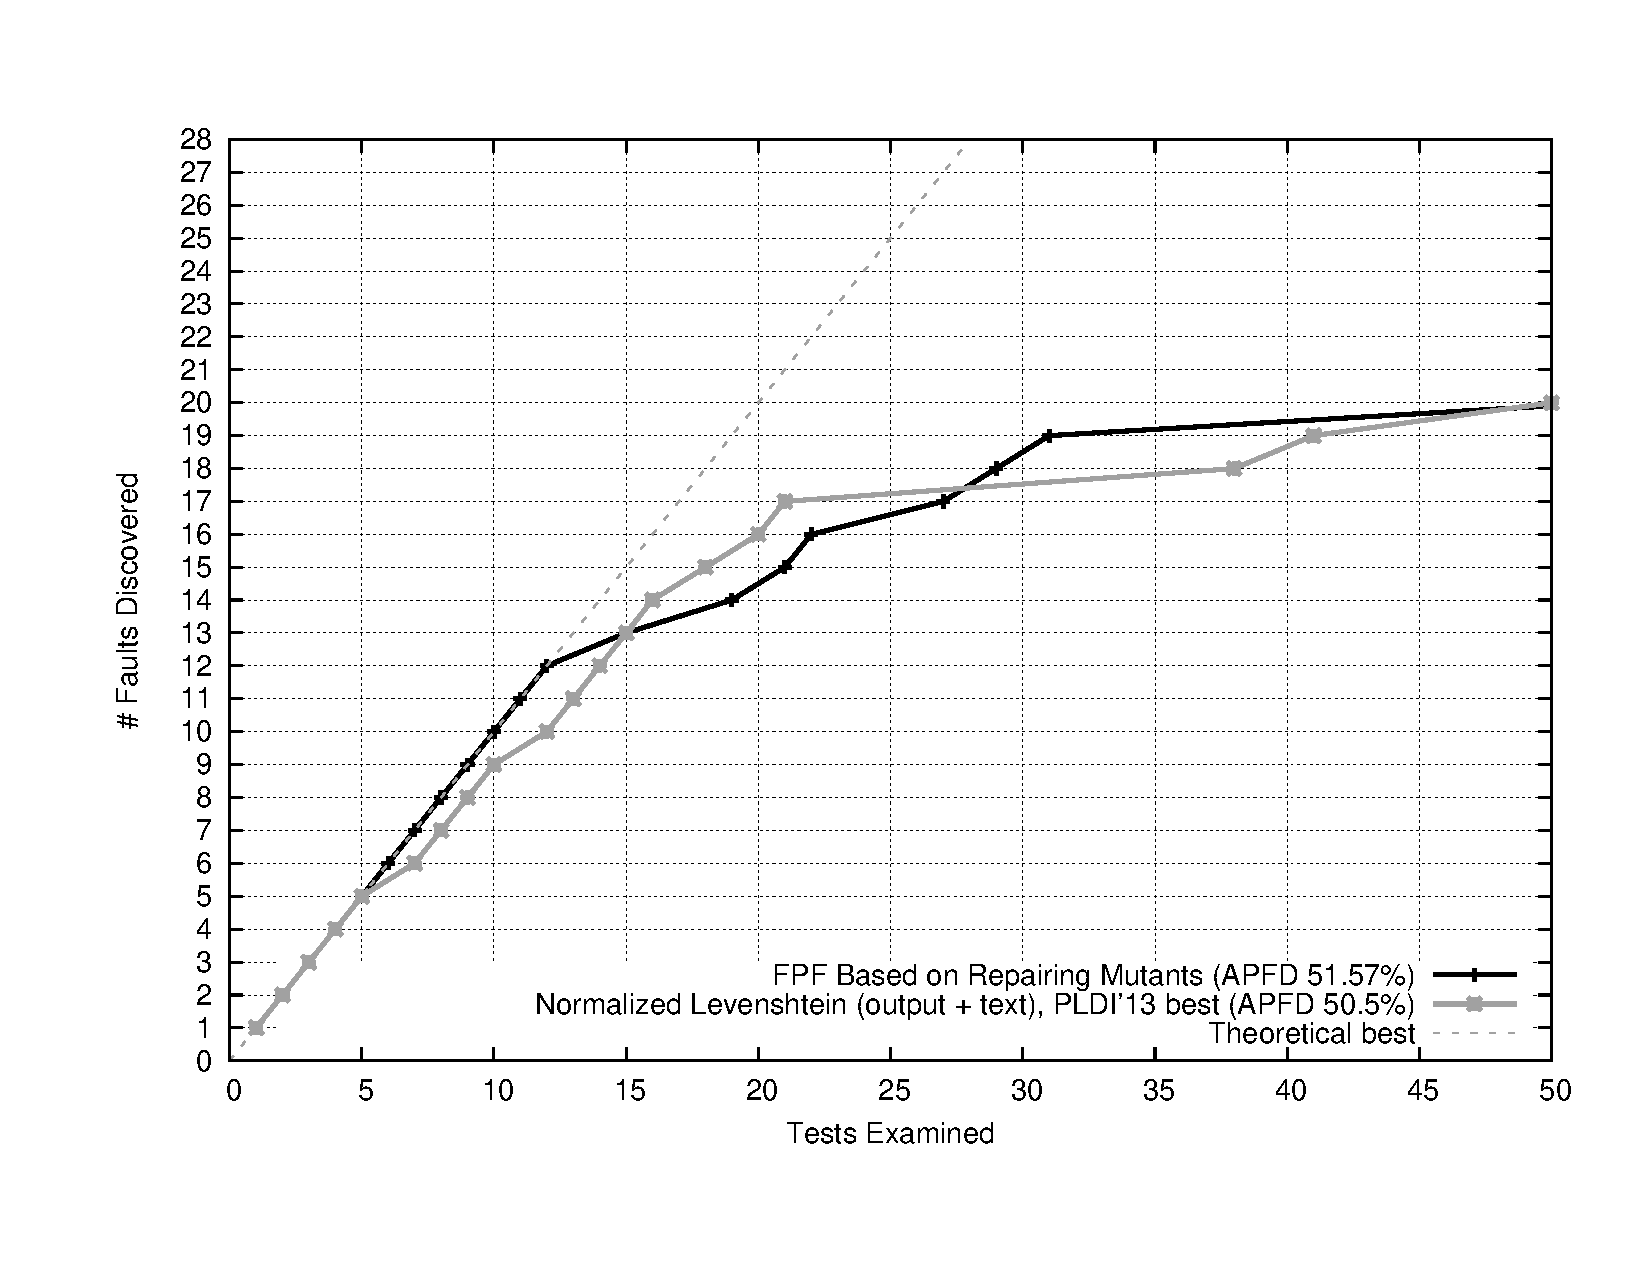
\includegraphics[width=2\columnwidth]{jscurve}
%\caption{Discovery curves for SpiderMonkey 1.6 faults}
%\label{jscurves}
%\end{figure*}


%\begin{figure*}
%\centering
%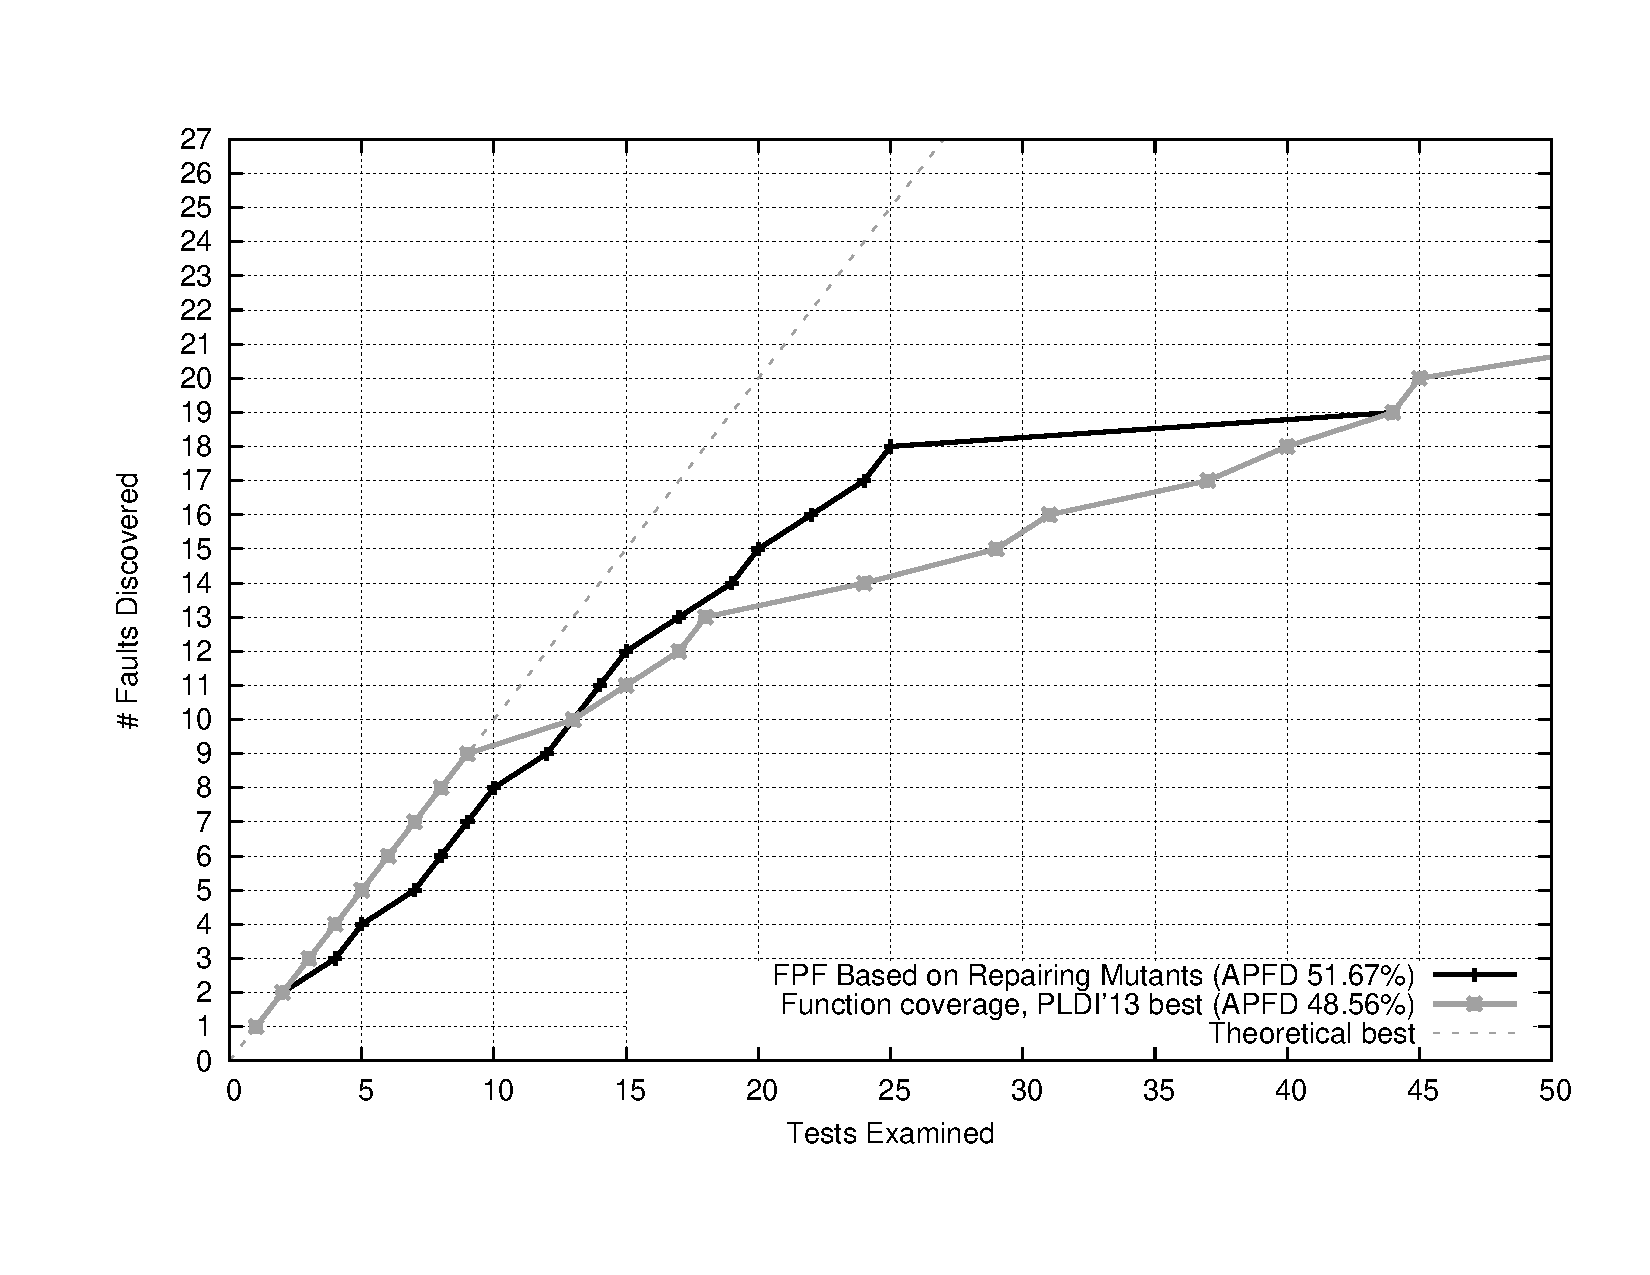
\includegraphics[width=2\columnwidth]{gcccurve}
%\caption{Discovery curves for GCC 4.3.0 wrong-code faults}
%\label{gcccurves}
%\end{figure*}

%\subsection{General Experimental Framework}

All experiments in this paper are based on subjects used in the only previous study of compiler fuzzer taming \cite{PLDI13}.  Of the three data sets examined in that paper, this paper considers two:  faults and tests cases for SpiderMonkey 1.6, Mozilla's JavaScript engine, with tests generated by {\tt jsfunfuzz} \cite{jsfunfuzz}, and \emph{wrong code} faults and test cases for GCC 4.3.0, with tests generated by Csmith \cite{csmith}.  GCC 4.3.0 crash faults were essentially perfectly localized by previous approaches.  Faults that produce a crash are also likely to be easier to debug than purely semantic problems, such as many of the SpiderMonkey faults and all GCC wrong code faults.

All mutants were produced using the C mutation tool written by Jamie Andrews \cite{mutant}, used in many previous experiments in mutation analysis and software testing.  Andrews' tool applies only four operators: statement deletion, conditional negation, operator replacement, and constant replacement, chosen as a small set that still produces good results for C code.  The tool was chosen to keep the number of mutants as small as possible to control the cost of mutation analysis.  Coverage was analyzed with gcov.   All experiments were performed on a MacBook Pro with 16GB RAM and dual-core 3.1GHz Intel Core i7 (not using the second core); GCC executed on a VirtualBox-hosted Ubuntu 11.04.  For GCC, some test cases from the 2013 PLDI paper no longer failed, presumably due to unknown differences in execution environment, OS, or memory layout. Discarding these reduced the set of test cases from 1,275 to 1,117 and the number of distinct faults to 27 rather than 35.  For SpiderMonkey, all 1,749 test cases from the PLDI 2013 data failed in the new environment, representing 28 distinct faults.

These data sets, though similar in that both compilers are written in C, provide some interesting variance for testing our hypotheses.  The oracle for SpiderMonkey executions is the set of checks built in to {\tt jsfunfuzz} plus the requirement that the execution not crash.   If the {\tt jsfunfuzz} produced test case executes to the end and prints {\tt TEST SUCCESSFULLY COMPLETED} it is considered successful.  This is only a moderately strong oracle, and allows serious deviations in behavior from both the JavaScript language specification and normal SpiderMonkey behavior, while constraining other some of execution fairly tightly, such as {\tt eval} round-trips.  For GCC, the oracle is a differential check on a hash code:  failure was defined as producing a executable with the -O3 flag that, when executed, produced a different checksum than code compiled by either of GCC 4.9.3 or clang 7.0.0, both using -O0.  A repairing mutant must enable GCC 4.3.0 to actually compile code correctly, which is a very strict correctness property in one sense, making coincidental correctness \cite{CCT} highly unlikely --- the only weakness is that there is no check that optimizations were applied, or that compile time was not excessive.

We only show results for the first 50 tests in the ranking, and computed areas under curves for the same limit, since it seems very unlikely that a user will examine many more than 50 tests, especially given the decreasing slope of the discovery curves.  In practice, after 50 tests, fixing a few faults and then re-running tests and FPF seems the most likely recourse, and we confirmed that after removing random subsets of faults, our metrics still outperform the previous best.  We applied X-means \cite{xmeans} in an attempt to use clustering, but, as with previous results \cite{PLDI13} clustering did not compare well with FPF, and the runtime was much worse than for FPF-based methods.  This tends to confirm earlier work's \cite{PLDI13} conclusion that clustering (at least based on X-means) simply does not work well in a setting with the kind of extreme disparity in instances of faults found in fuzzer taming.  A further difficulty for our setting is that X-means and most off-the-shelf clustering tools take vectors, not a distance metric.  X-means is using the raw repair data, not weighted by the fact that 0-0 agreement is much less informative than other possible matchings (recall that a Euclidean over 0-1 vectors is just the square root of Hamming distance).

\subsection{Mozilla SpiderMonkey 1.6 Results}


There were 96,828 SpiderMonkey mutants, based on 69,634 lines of code in C and header files.  Of these mutants, 12,666 were covered by some failing test case.  Of these mutants, 10,525 survived a basic set of SpiderMonkey quick tests \cite{icst2014}.  Of these mutants, 1,326 (12.6\%) repaired at least one test case.  Figure \ref{jscurves} shows the discovery curves for the mutant repair metric compared to the ideal discovery curve and the best curve from previous work using FPF, which used a normalized Levenshtein distance \cite{lev} over the failure output and test case text \cite{PLDI13}.  The APFD (Average Percent Faults Detected) values shown in the graphs are based on the measure  introduced by Rothermel et al. to evaluate test case prioritization methods \cite{APFD}.  This is a somewhat better summary of results than the raw curve areas used in previous work \cite{PLDI13}.  APFD, as the name suggests, shows the percent of all faults discovered at the ``average'' point on the curve, by comparing the curve's overall area to an ideal curve, with interpolation\footnote{The details of APFD calculation are slightly involved, and the interpolation and perfect curve are not exact fits for fuzzer taming; nonetheless the basic method summarizes curves fairly well and is standard in the testing literature for similar problems \cite{issta14}.}. 

APFD results are useful summaries, but we suggest that the curve itself is also worth examining, since (1) a very good early curve is perhaps most important to developers and (2) long sequences of tests with no new faults may discourage users more than an overall less effective but steadily climbing curve with few ``plateaus'' as we call these uninformative sequences of tests.  The SpiderMonkey curve climbs very rapidly in the early portion, with perfect discovery for the first 12 faults. The largest plateau is 5 tests without a new fault, ignoring the long period after the 31st test.  In fact, a plateau at the end of the curve is not problematic.  Assuming that few users will examine more than 50 test cases without fixing some faults, the user may give up after seeing 10 or more tests without a new fault based on the mutant repair curve, and in fact lose nothing by doing so.  The PLDI 2013 curve, in contrast, has a plateau of size 17 after the 17th fault.  If we assume a user stops examining tests after a size 10 or greater plateau, the user will only see 17 faults using the PLDI 2013 metric, vs. 19 with our metric.  Dropping the stopping criteria to a plateau of size 5 produces the same results.

Over all mutants, and all pairs of test cases repaired by the same mutant (so the same pair may count many times, if many mutants repair both test cases), the probability of being due to the same fault was 42.77\%, and the probability of being due to the same fault if two test cases disagreed on a repair (the mutant repaired one test case but not the other) was only 20.33\%.  The baseline rate for same-fault for test pairs was 33.64\%.  Just knowing that two test cases have \emph{one} shared repairing mutant makes it 1.27x more likely that they are the same fault, and knowing they differ for one mutants makes it 0.6 times as likely they are due to the same fault.  As suspected, while matching non-repair provided some evidence, that evidence was quite weak:  only a 34.14\% chance of matching fault.

An additional measure of effectiveness is to consider how effective a metric is in producing matched nearest neighbors.  That is, how often is the nearest neighbor of a failure (that is not due to a singleton fault --- a fault detected by only one test case) due to the same fault?  For reduced \cite{DD,PLDI13,
CReduce} test cases, we assume that for a perfect metric, the nearest neighbor should almost always share the same fault, since there is little or no extraneous semantic content to each test beyond the cause of failure.  For the SpiderMonkey failures, 96.3\% of non-singleton failures matched their nearest neighbor(s).  For mutants that repaired any failures, the mean and median number of test cases repaired were 120.6 and 4.0, respectively.  Most mutants repaired a small number of tests, but a few mutants repaired a very large number of tests.  A few mutants repaired \emph{all} SpiderMonkey faults; obviously these mutants were not actual fault fixes of any kind, but effectively disabled some mechanism {\tt jsfunfuzz} used to detect failure. The mean and median homogeneity for repairing mutants (percent of failures repaired corresponding to the most common fault repaired) were 77.96\% and 86.36\%, respectively.  

\subsubsection{Fault Localization}

Table \ref{jstable} shows a comparison of three fault localization methods for the SpiderMonkey faults.  The first column shows, for each fault, identified by the commit number of the code change that first ``fixed'' the failing tests associated with the fault, its FPF ranking: this is \emph{not} a fault localization ranking, just a way to see that the localization success seems to be somewhat independent of the ease of distinguishing the failures for a fault.  The next four columns show localization rankings.  A dash for a column means that localization did not rank any faulty statements, or assigned all faulty statements suspiciousness of 0.0.  The four rankings are: the {\bf Coverage} localization, the {\bf Repair} localization, the MUSE \cite{MUSE} localization, and the MUSEUM \cite{multilingual} localization, which uses the same formula as MUSE, but works better for multiple faults because it uses only one failure.  The MUSE/MUSEUM formulas normally make use of information from passing tests as well: when mutating a statement makes a passing test case fail, it makes the statement \emph{less} suspicious, by a weighted amount. The weight assigned to information from passing tests in our setting would likely be low (due to the ratios of repairs to mutation kills).  In a limited sense, information from passing tests is already incorporated in our results.  Throwing out all mutants that are killed by any passing test as potential repairs/localizations ensures that the rankings of all statements that are in MUSE/MUSEUM rankings are correct, relative to each other.  By definition, passing tests have no influence on the suspiciousness of these mutants.  However, there may be other mutants that 1) repair a failure and 2) are killed by some test case: these could, if enough repaired a faulty statement, improve MUSE/MUSEUM results.  We reject such mutants in part to keep costs low, and in part because we think that the causal information contained in such mutants, that repair a failure but also break some passing test, is problematic.  They seem likely to be less useful as explanations of the causes of a failure, since they do not impact the program semantics in a way that is only known to be beneficial, and could potentially even mislead a user if used as explanations.

Discussion with the MUSE/MUSEUM authors confirms  that adding information for passing tests, while costly, would likely improve the MUSE and MUSEUM results, given the weakness of our oracles, particularly for SpiderMonkey, and should be considered essential for ideal application of their approach.  Because the cost of recording the full mutant analysis matrix for all passing tests (rather than considering a mutant killed as soon as one test fails, as we do) is very high, and we would like to produce a comparison over a fixed computational cost, we give results for MUSE/MUSEUM over failing tests only, cautioning that we are not sure what the impact of this choice is.  For similar reasons of keeping costs low, we also used the mutation operators of Andrews vs. the more extensive Proteum \cite{Proteum} operators used in MUSE/MUSEUM's evaluations.  Even with these restrictions, running all mutants on passing tests took about 3 times as long as the search for repairs, which we already consider a potentially problematic cost.

Results are reported as absolute ranks, rather than more sophisticated \cite{MUSE} localization evaluations because our localizations do not assign suspiciousness scores, only rankings, and in accord with the proposal of Parnin and Orso that only localizations ranking a fault in the top few statements may be useful to users \cite{AutoHelp}.  We expect users to examine coverage changes and mutants.  Blind, unaided pointers to portions of compiler code without more semantic information about why the statement is suspicious seems unlikely to work well, based on our experience with complex compiler faults, and the results of Parnin and Orso \cite{AutoHelp}.

\begin{table}
\centering
{\scriptsize
\begin{tabular}{|c||c||c|c|c|c|}
\hline
& & \multicolumn{4}{|c|}{Localization Rank} \\
\hline
Fault & FPF & Coverage & Repair & MUSE & MUSEUM \\
\hline
880 & 1 & 2,255 & - & - & - \\
95 & 6 & 720 & - & 173 & -\\
1294 & 9 & 190 & 1 & 22 & 4 \\
60 & 10 & - & - & - & -\\
1543 & 15 & 18 & 19 & 118 & 26\\
1172 & 19 & 46 & 28 & 87 & 23\\
1561 & 106 & - & - & - & - \\
115 & 192 & 6 & 3 & 133 & 5 \\
\hline
\end{tabular}
}
\caption{Fault localization results for SpiderMonkey}
%\vspace{-0.2in}
\label{jstable}
\end{table}


\begin{figure}
{\scriptsize
\begin{code}
{\bf Diff of old ($<$) vs new ($>$) for 115 patch (portion):}
...
<             vp[1] = OBJECT\_TO\_JSVAL(thisp);
<         \} else \{
<             ok = OBJ\_GET\_PROPERTY(cx, thisp, id, \&v);
<         \}
...
<                   a->avail = (jsuword)sp;
<               \}
...
---
>         RESTORE\_SP(fp);
...
{\bf Mutant information:}
Failure repaired by 148 mutants.
...
\#3: delete statement mutant of jsinterp.c:944:

            vp[1] = OBJECT\_TO\_JSVAL(thisp);
        \} else \{
/*MUTANT    ok = OBJ\_GET\_PROPERTY(cx, thisp, id, \&v);*/
        \}

{\bf Coverage change information:}
...
\#6: 5 mutants (3.38\% of repairs) added jsinterp.c:992:
                   a->avail = (jsuword)sp; /* ADDED */
\end{code}
}
\caption{Patch and explanation for fault 115}
%\vspace{-0.18in}
\label{fig:explain}
\end{figure}

The first thing to note about results is that Table \ref{jstable} only includes 8 of the 28 SpiderMonkey faults.  This is due to a problem discussed in the paper introducing this data set:  producing ground truth patches for a large application, in the sense of finding a minimal, clearly fault-fixing code change that can be back-ported to the original code is difficult \cite{PLDI13}.  While we believe the 28 faults identified in the PLDI 2013 data set are correct, it is very difficult to produce a valid patch of version 1.6 that captures the fix for most of these faults.  In some cases the final commit that caused tests to stop failing appeared to only be the end of a complex series of changes that converged on a correct fix.  In other cases, the code was modified so extensively before the fix that identifying ``the incorrect part'' of the original code seemed to owe more to guesswork than certainty.  The evaluation of localization therefore only examines the 8 faults for which we could be reasonably certain that the patch to 1.6 was correct and characterized the fault in question accurately.  The smallest patch required modification of two statements, and was thus larger than any mutants applied.  In no case was the patch equivalent to one of the mutants.

No method performs extremely well --- for half the faults, no methods produced what we consider a useful localization.   Compiler faults are hard to debug, and any help is useful, but it seems unlikely developers will really benefit from a localization when it does not rank at least one faulty statement in (at most) the first 20 to 30 statements.  By this measure, MUSE only provides a helpful localization once, and performs worst of the methods.  {\bf Coverage} performs very badly for three faults, and does not manage to be useful by our definition for another, but in the remaining two cases provides a good localization, in one case the best.  {\bf Repair} and MUSEUM both perform well, with {\bf Repair} slightly better.


\subsubsection{Error Explanation}


Figure \ref{fig:explain} shows part of the patch for SpiderMonkey fault 115, and the {\bf Coverage} and {\bf Repair} outputs that successfully localize the fault (the 6th coverage change output, and the 3rd mutant output), to give some idea of the information our methods present.  For {\bf Coverage}, it is surprising that the sixth highest ranked change only appeared in 5 of 148 repairs. This change ranked high out of thousands of coverage changes because it was an unusual coverage change, appearing for only 10 repairs in the entire SpiderMonkey analysis. 

The precise form an explanation based on our techniques should take is not clear.  One possibility, suggested by the results here, is a method focused on repairs, but using common coverage changes.  For each repairing mutant, in rank order, the highest ranking coverage changes for that mutant could also be shown, to give an idea of unusual (and potentially localizing) changes induced by repair.


\subsection{GCC 4.3.0 Wrong Code Results}


There were 377,679 GCC mutants, based on 424,186 lines of code in C and header files. Of these mutants, 73,016 were covered by some failing test case.  Of these mutants, 41,385 survived a GCC bootstrap build (used to produce our compiled versions for repair checks), compiled hello world correctly, and passed a GCC test suite.  Of these mutants, 3,232 (7.8\%) repaired at least one test case.  Figure \ref{gcccurves} shows discovery curves for the mutant repair metric vs. the best PLDI 2013 curve, Euclidean distance over function coverage vectors \cite{PLDI13}.  GCC's APFD improvement is larger than that for SpiderMonkey, but its early curve is worse compared to the PLDI 2013 curve.  Using the hypothetical model where a user stops examining tests after a plateau of size 10, the user of the mutant-based taming will see 18 distinct faults by examining 25 tests, and the user of the function coverage based taming will see 20 faults after examining 45 tests.  If a user gives up after a plateau of size 5, our approach again lets a user examine 18 faults over 25 tests.  Function coverage provides only 16 faults over 31 tests. 

For GCC wrong code faults, the baseline chance two test cases shared an underlying fault was 38.97\%.  Knowing that two test cases shared a repairing fault raised the chance to 68.5\%, and knowing they disagreed on a fault lowered it to only 19.01\%.  The respective increase and decrease in probability of matching fault compared to baseline was thus 1.75 times greater for matching repairs, and less than 0.5 the chance of being the same fault, given one mismatched repair.  Knowing two test cases were both not fixed by a mutant again provided marginal evidence of sharing a fault: 39.2\% chance of matching faults.
For 99.3\% (all but 8) of the 1,090 non-singleton fault failures in GCC wrong code, the closest test case(s) by the repair metric matched fault.  The best previous reported FPF metric, function coverage vectors, had a matching rate of 92.2\%.   The mean and median numbers of repaired tests per mutant (for mutants that repaired any tests at all) were 18.4 and 3.0, respectively.  A few mutants fixed a very large number of tests, up to 1,050\footnote{These all appear to be turning off all optimizations --- forcing GCC to run in -O0 mode.}, but most mutants fixed only a few tests, to a greater extent than was true with SpiderMonkey.    The mean and median homogeneity (\% of repaired tests corresponding to the most commonly repaired fault) were 79.4\% and 100\%, respectively --- over half of all repairing mutants only repaired instances of the same fault.  

\subsubsection{Fault Localization}

\begin{table}
\centering
{\scriptsize
\begin{tabular}{|c||c||c|c|c|c|}
\hline
& & \multicolumn{4}{|c|}{Localization Rank} \\
\hline
Fault & FPF & Coverage & Repair & MUSE & MUSEUM \\
\hline
139094 & 1 & 44,561 & - & 157 & -\\
133004 & 2 & 75 & 1 & 99 & 14\\
158782 & 4 & - & - & 146 & -\\
156496 & 5 & 3,067 & - & - & -\\
143677 & 7 & 186 & - & 109 & -\\
158555 & 8 & 490 & - & - & -\\
134321 & 10 & - & - & - & -\\
133940 & 14 & 260 & 4 & 158 & 18\\
141195 & 15 & 465 & - & - & -\\
156795 & 17 & 19 & - & - & -\\
139709 & 19 & 43,903 & 10 & 167 & 6\\
155698 & 22 & 85 & 1 & 172 & 195\\
138646 & 24 & 2 & - & - & -\\
140795 & 25 & 302 & 34 & 170 & 125\\
136501 & 44 & 223 & 5 & 159 & 31\\
134322 & 45 & 639 & - & - & -\\
\hline
\end{tabular}
}
\caption{Fault localization results for GCC}
\label{gcctable}
\end{table}

Table \ref{gcctable} shows localization results for GCC 4.3.0 wrong code faults.  For the same reasons as with SpiderMonkey, only some faults were deemed to have a strong enough ground truth patch for localization evaluation.   MUSE performed poorly, with no useful (by the standard of having at least one faulty statement in the top 30) localizations.  {\bf Coverage} produced one very good localization, and was the only method to localize that fault at all, but this was its only useful localization.  MUSEUM provided two respectable localizations, but no very high quality localizations.  Only {\bf Repair} performed extremely well:  while it only localized three faults, those localizations were all extremely useful.

\subsection{Discussion}

In one sense, the discovery curve improvements here are practically useful, but not spectacular.  The SpiderMonkey curve has an APFD only slightly more than 2\% better than the best result from previous FPF efforts.  The GCC wrong code curve improves APFD by 6.4\%.  However, the comparison is with the very best curve chosen after running more than 16 different metrics.  In practice, users do not know ground truth to rank competing curves, so this is not a practical approach to fuzzer taming.  The best methods for different subjects in previous work varied widely, even in such peculiar ways as less-fine-grained coverage providing better results in some cases, worse in other cases.   In practice, previous work established that FPF could produce good curves, but gave very little useful guidance for choosing a metric for actual use of the technique, and included methods such as comparing output signatures that are inapplicable to many settings.  This paper presents a single curve using a universal metric, and achieves a 2-6\% percentage point improvement over the best of more than 16 different metrics studied in the previous work.

For fault localization and error explanation, the results show possible improvement on state-of-the-art approaches, in the absence of complete information from mutant analysis over passing tests (which can be very expensive to obtain).  A practical impact of the results reported is that we suggest users of our techniques examine only the first few (at most 10, and we propose as few as 5) mutants and coverage-changing statements, and ignore localization if none of these results are helpful.  This is analogous to our suggestion that a user abandon the FPF curve if 5-10 test cases in a row fail to reveal any new faults, as a heuristic.  We suspect the information in the mutants/coverage changes is probably helpful in some cases where they do not localize a faulty line, but this is simply based on our highly incomplete understanding of the faults and patches in question, and not a solidly established claim.  The expertise of compiler developers would be needed to confirm or reject this belief.  Our suggestion that mutations themselves provide interesting error explanation is also applicable to MUSE and MUSEUM.  There may be some potential for confusing explanations, however, if repairs include mutants that also cause some failures, as in the standard MUSE/MUSEUM approach.

One obvious question is:  why does {\bf Repair} perform best in this setting?  It is impossible to be sure, but one  possibility is power to distinguish repairs. If each failure was only repaired by one mutant, MUSEUM and {\bf Repair} would both rank that mutant maximally, and we speculate it would usually be faulty.  But such cases are rare:  for SpiderMonkey the mean/median number of mutants repairing each failure were 90.8 and 78, respectively, and for GCC the mean and median were 54 and 43.  If there are many repairs for a failure, how can the most important ones be distinguished?  MUSEUM relies on a large set of mutation operators, and assumes that faulty statements will have multiple repairs, compared to non-faulty statements, or that faulty statements will be less likely to cause passing tests to fail when mutated.  Restricting ourselves to cases where {\bf Repair} and MUSEUM both provided a localization, we know that some faulty statement was in a repairing mutant, but that passing tests could not distinguish this mutant  from other repairs.  Many of the faulty statement repairs (as expected for optimizing compilers) were statement deletions and conditional negations.  For these, it seems unlikely that Proteum would produce more mutants repairing the statement, though perhaps Proteum would create repairs for other statements that cannot be modified into a repair by any of Andrews' operators.  {\bf Repair} can still distinguish such mutants by relying on the onion-ring structure:  when a repair also repairs test cases that otherwise do not resemble the failure being localized (in terms of its repairing mutants), {\bf Repair} assumes that repair is general to many different faults.  The hypothesis behind {\bf Repair} is that \emph{repairs specific to the fault causing a failure are most likely to modify code involved in the fault itself}.  This seems to be true, when such a repair exists.  If any repair for a failure modified a faulty statement, {\bf Repair} always ranked it in the top 34 localizations, ranked it in the top 5 in 6 of 10 such cases, and 3 times ranked it 1st.  MUSEUM, in contrast, ranked one such repair 195th, never ranked a fault in its top 3 statements, and only ranked a fault in its top 5 statements twice.  Of course, MUSEUM might be suffering from a lack of mutation operators, but in some cases this is unlikely due to the nature of the repairs.

Finally, in contrast to many previously reported results in fault localization, typically over much simpler programs and faults than subtle compiler semantics bugs, all methods frequently failed to provide a useful localization at all.  In one sense, {\bf Coverage} is the most intriguing method presented here.  While it did not perform nearly as well as {\bf Repair}, it did manage, in many cases, to rank some faulty line highly relative to the extremely large number of statements executed in each failing GCC run (on the order of 50K-100K+ statements).  In future work, we plan to experiment with different methods for weighting frequency of coverage, perhaps using methods from machine learning, or of pruning changed coverage that is not likely to be relevant.  For example, perhaps the {\bf Repair} approach can be applied, and coverage changes present in very distant failures can be removed, though the argument is less clear, since a coverage change isn't directly associated with the onion-ring structure, and does not directly repair a set of failures.  There is much to be done if automated debugging is ever to make the lives of compiler developers easier in most cases \cite{AutoHelp}.  

\subsubsection{Mutation Analysis Costs}

Mutation analysis is not cheap.  The experiments in this paper were run over a long period of time.  However, there are numerous ways to reduce costs.  First, the primary cost is compiling the mutated versions of the SUT.  Running each test case under each mutated version of the compiler is cheap: each execution requires around 0.05 seconds for SpiderMonkey, and 0.12 seconds for GCC, on average.  These executions can obviously be performed in parallel, on low-cost virtual machines in the cloud.  The cost is further reduced by a few more facts: most failures do not cover most mutants, and vice versa, so the total number of repair checks needed is far less than the product of mutants and failures.  The practical approach to fuzzer taming for a large, ongoing project is likely to maintain a set of ``hot'' pre-compiled mutants.  These can be pruned at will by running them on passing test cases, and removing mutants that fail on any test case.  Keeping hot mutants for a heavily modified program could be costly (since each mutant must be recompiled, if not re-tested, for each modification to the code), but for stable releases this is a simple approach to keep costs low.

Second, and most critically, most program mutants never need to be considered as repairs, because we only consider mutants that cause no passing test case to fail.  MUSE and MUSEUM use kills by passing tests to help rank such tests as repairs, which is finer grained but more expensive.  As we show, MUSE and MUSEUM \emph{can}  be used without passing tests or these mutants, and MUSEUM still produces good results even with a weak oracle and few operators.  MUSE, MUSEUM, and our approach all run analysis without coverage instrumentation; we re-run repaired tests under gcov when using the {\bf Coverage} localization.

Mutation cost reduction techniques are also applicable.  E.g., trivial compiler equivalence (TCE) \cite{TCE} can reject equivalent and redundant mutants, removing almost 30\% of mutants for benchmark subjects. Other techniques, such as using mutant schemas to avoid having to compile and store each mutant, are also applicable --- almost all of the techniques characterized by Offutt and Untch \cite{offutt2001mutation} as \emph{do faster} approaches apply.   Whether sampling mutants \cite{RahulISSRE} is applicable is less clear.  Even if the FPF curve remains the same, a critical mutant for localization might be omitted.

\subsection{Threats to Validity}

The largest threat to validity is that this paper's conclusions rely on only two data sets, used in a previous paper.  The fault ground truths are possibly imperfect, due to the complex change history, and it was not possible to produce good patches for all faults, limiting our analysis of localization and explanation.  Generalizing to all compilers, or to software systems that are not compilers, would be unwarranted.  However, for compilers, we believe the underlying arguments supporting the probability of discovering many meaningful repairing mutants should hold in the general case.  There is no particular reason to believe that Csmith and {\tt jsfunfuzz} produce unusual random test cases, and both have often been used to detect faults in compilers other than the two considered in this paper.  For other kinds of software, more experiments are definitely warranted.  It is also possible that faults in the framework used for experiments introduced errors into the data.  In order to check for these problems, we will make the raw data for a re-analysis available on request.

Second, the comparison with MUSE and MUSEUM is limited.  MUSE is not really intended for multiple faults.  With our oracles, MUSE and MUSEUM may need the full results from passing tests, and some mutant we omit might be both highly ranked and a good localization.  A full comparison would include a complete analysis of passing tests also, but would likely require far more than 10x the computation time.  Finally, these experiments use Andrews' mutation operators, while MUSE/MUSEUM experiments use Proteum \cite{Proteum}, which has a much larger set of mutation operators, and their results indicate that the large set of operators is important.  However, running all Proteum GCC mutants (especially over all passing tests) would likely be very expensive.
